\chapter{Software Design}
\label{ch:ch5}
This chapter outlines the software design methodology for the SHARC buoy based on the hardware design and components selections in Chapter \ref{ch:ch4}. This chapter describes the firmware written for SHARC buoy version 2. This version contains the STMicroelectronics STM32L476RG 32-bit microcontroller, \cite{stm32l4} which contains the Arm Cortex-M4 processor \cite{ARMprocessor}; a low powered 32-bit microcontroller, based on the Armv7E-M central processing unit (CPU) architecture and Harvard bus matrix architecture. A high-level overview of this microprocessor is shown in Figure \ref{fig:cpu}.

\begin{figure}[H]
	\centering
	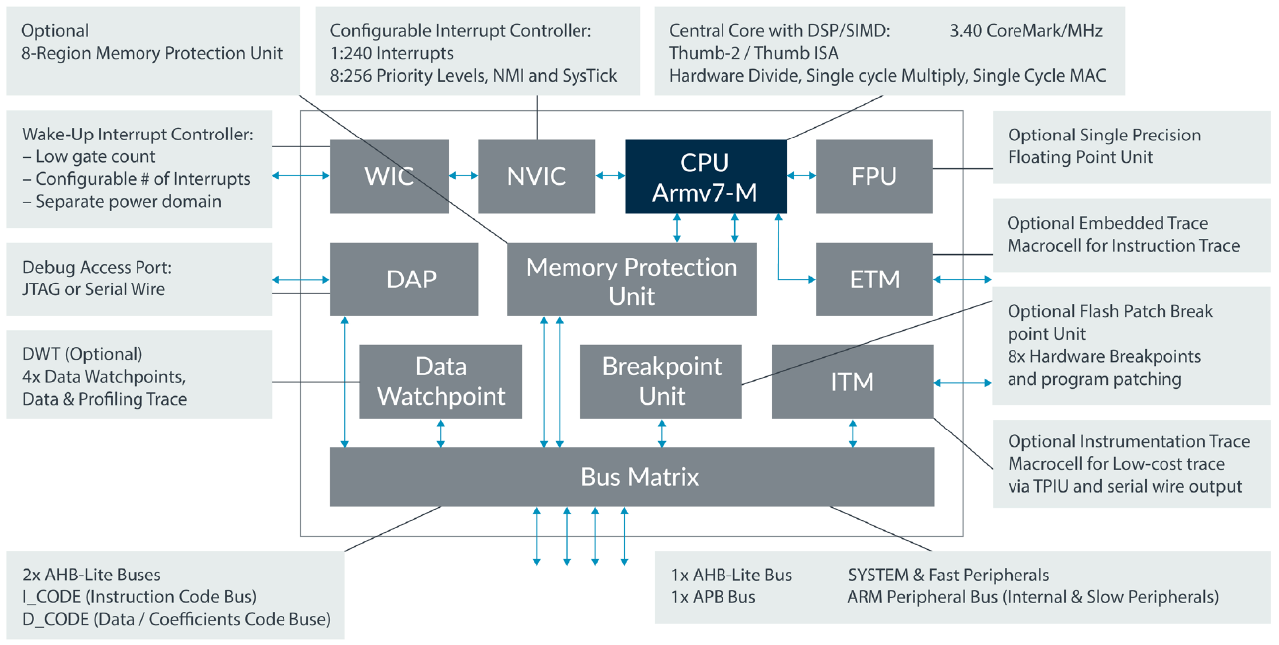
\includegraphics[width = \textwidth]{cpu_architecture.png}
	\caption{Block diagram of the Advanced RISC Machines (Arm) Cortex-M4 microprocessor. This device features a Harvard bus matrix and Armv7E-M central processing unit. The processor also contains a hardware floating point unit (FPU), nested vector interrupt controller(NVIC) for controlling interrupts and a wakeup interrupt controller (WIC) for low power operational control. This processor can be programmed through serial wire via STLink or via JTAG. Image source: \cite{ARMprocessor}. }
	\label{fig:cpu}
\end{figure}

The software was compartmentalised to improve the modularisation of the firmware. This accommodated changes to the hardware subsystems during the development stages without writing entirely new software. Compartmentalisation was also necessary to accommodate microcontroller changes as the new microcontroller had a different pin map and processor architecture to the previous version of the buoy. The project was initially developed in C using the STMicroelectronics standard peripheral libraries (SPL). However, in 2019, these libraries had depreciated and were replaced with the STMicroelectronics Hardware Abstractionion Layer (HAL) libraries. This change also resulted in a change in firmware architecture due to a difference in the software project structure. Therefore, this section will focus solely on the firmware design for version 2 of the buoy.

This chapter begins with an overview of the development environment, tools, and libraries used to develop the firmware. An overview of the firmware architecture is presented, showing the layers and sections of the firmware. The timing requirements are presented, followed by the configuration parameters for the system clock real-time clock (RTC). These are followed by a discussion of the effects of these configurations on the overall system. Next, the software power optimisation techniques are presented, showing the selection of a suitable power mode and the impact during runtime. The main software is presented, showing careful consideration of timing requirements and the synchronous, and asynchronous behaviour during run time. The chapter closes with the systems data requirements followed by the techniques used to manage data between subsystems and data transfer from the device to a user.

\section{Software architecture}

The STMicroelectronic STM32 microcontrollers do not come loaded with any operating system. Therefore, firmware development had to occur at the base level. In addition, the firmware had to be tailored to the specific microcontroller architecture. A decision was made to write the firmware in C as it allowed for higher-level code to be implemented while still optimising for size and speed on the device. The Atollic Truestudio integrated development environment (IDE) allowed for development to take place in C/C++. This development platform includes an integrated Arm development tool chain and a GCC compiler allowing for easy code compilation and device programming via a USB cable. STMicroelectronics also provides a set of driver files and tools to assist with peripheral initialisation which reduced development time. \par 

The firmware was designed using a top down approach. The overall system was decomposed into three distinct layers as shown in Figure \ref{fig:soft_arch}.

\begin{figure}[H]
	\centering
	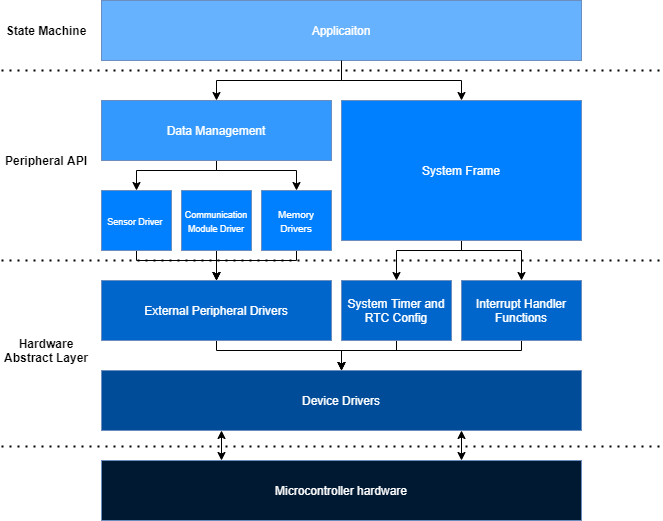
\includegraphics[width= 0.7\linewidth]{soft_arch.png}
	\caption{Diagram showing the decomposition of the overall firmware into distinct layers and the relationship between each part.}
	\label{fig:soft_arch}
\end{figure}

Figure \ref{fig:soft_arch} provides the basis for the firmware development. The main application is built on supporting layers with each layer providing an interface for a level closer to the hardware. These layers are discussed in Subsection \ref{subsec:ch5_hal} to \ref{subsec:ch5_SML}. 

\subsection{Hardware abstraction layer}
\label{subsec:ch5_hal}
The hardware abstraction layer (HAL) consists of the driver files used to initialise and control the hardware of the microcontroller. This layer is processor specific and therefore needs to be tailored to the architecture of the selected microcontroller. This layer comes pre-written as a set of library files provided by STMicroelectronics which were included in the Atollic Truestudio IDE. The STMicroelectronics STM32L4 Standard Peripheral Library (SPL) was first used as the hardware abstraction layer in version one of the firmware. However, in 2019, the library had depreciated and was replaced with the STMicroelectronics Hardware Abstraction Layer (HAL) libraries. HAL libraries were used to form the foundation of the code as it allows for the code functionality to run independently from the hardware architecture. Should a new microcontroller be required, the HAL library simply needs to replaced. Therefore allowing the firmware to maintain modularisation and increase portability. In addition, the HAL libraries offers robust error checking and flagging. If a peripheral fails at any point during run time, the libraries provide handlers and flag signaling to handle the error.

\subsection{Subsystem application peripheral interface (API) layer}

Next, hardware-specific driver files were written for each subsystem. These files formed the subsystem application peripheral interface (API) layer shown in Figure \ref{fig:soft_arch} which interfaces with the hardware peripherals through the HAL layer thereby reducing dependencies on the hardware. In addition, these driver files were created to abstract the initialisation and configuration process of each peripheral as well as the hardware routines that occur. Some external modules required the use of more than one peripheral such as timer channels for input capture or general purpose input/output (GPIO) pins for external interrupt detection. Finally, these drivers are critical for managing the flow of data too and from the module. Furthermore, these files contain functions that interpret incoming data bytes and convert them to the relevant data type.

\subsection{Main program layer}
\label{subsec:ch5_SML}
The state machine layer is the highest level layer of the firmware architecture shown in Figure \ref{fig:soft_arch}. In this layer the configuration files and other libraries are synthesised and sequenced into one main program. This program is responsible for controlling sensors and implementing data processing functions. This layer interfaces with sensor APIs through routines. Functions written in this layer are designed to control the behaviour of peripherals. For example, implementing a routine to initialise a sensor, sample the sensor and then turn it off. Further details of the main program will be discussed in Section \ref{sec:ch5_projstruct}.

\section{Project structure}
\label{sec:ch5_projstruct}

In this section, the tools used to develop the software are given. A description of the project files and project organisation for the main program, auxiliary files and libraries is provided.

\subsection{Project tools and files} 

The project was set up using STMicroelectronics STM32CubeMX. This is a tool for creating an embedded firmware project that generates platform-specific intialisation code and creates a project folder with peripheral initialisation and handling functions. This tool was used to quickly set up a project as well as configure the clock settings and include the correct HAL libraries. The project code files are organised into the following folders:


\begin{enumerate}
	\item Drivers
	\item Source (src)
	\item Start up 
\end{enumerate}


The drivers folder contains the HAL and Cortex microcontroller software interface standard (CMSIS) libraries for the device. These are a set of processor-specific libraries for the Arm cortex processor which provide a higher level interface between the microprocessor hardware and the firmware (see Figure \ref{fig:soft_arch}). The source folder contains the main.c file which acts as the entry point for the program to run. The start up file contains assembly code that specifies the vector table, hard fault/reset handler entry Points as well as the entry point for the main code. 

\subsection{Program startup and entry}

Program execution begins with the file \textit{startup\_stm32l476xx.s}. This is an assembly file that initialises the volatile (RAM) and non volatile (FLASH) memories and the main stack pointer (MSP) in the CPU. The file also contains:

\begin{enumerate}
\item Reset handler
\item Hard fault handler
\item Non maskable interrupt (NMI) handler
\item Interrupt vector table
\end{enumerate}

Resets, hard faults, watchdog events and non maskable interrupts are critical interrupt events that cause the main program to halt execution. Hard faults and non maskable interrupts come from run time exceptions that result in critical failures while resets cause the microcontroller to restart code execution. The interrupt vector table contains references to interrupt handlers from interrupt requests generated by the NVIC. If the start up file executes successfully, the microcontroller will load the \textit{main.c} and begin the main program. This program flow is shown in Figure \ref{fig:progflow}.\par 

\begin{figure}[H]
	\centering
	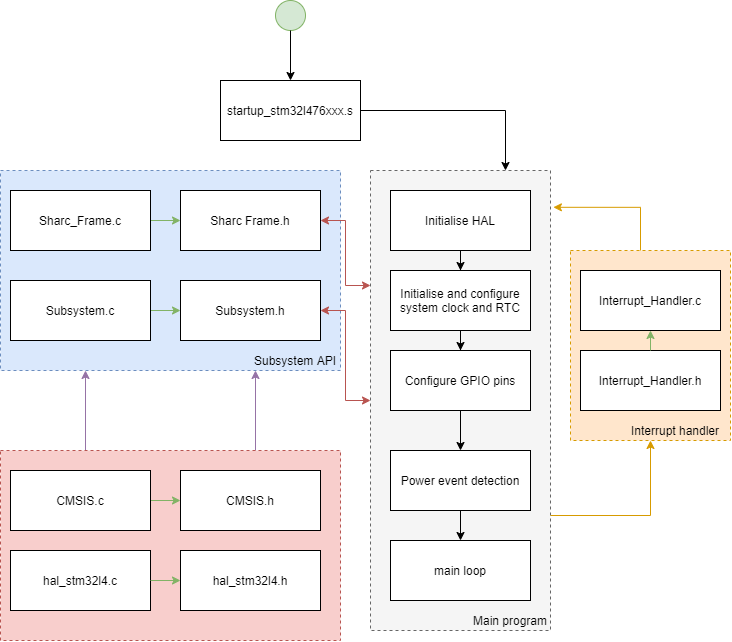
\includegraphics[width=\textwidth]{projflow.png}
	\caption{Diagram showing the firmware execution from (green) start. On start up, the \textit{startup\_stm32l476xx.s} file executes and loads the main program. This program runs in a continuous loop until the power supply to the device is turned off. This diagram shows the interaction of the firmware layers (see Figure \ref{fig:soft_arch}): (blue) subsystem API, (red) HAL and (grey) the main program. Also shown are arrows indicating (black) the main flow of the program, (green) references to functions, (red) calls to function prototypes and (orange) interrupts.}
	\label{fig:progflow}
\end{figure}

The program enters into the \textit{main()} function which marks the start of the main application. Figure \ref{fig:progflow}. The source folder contains the \textit{Sharc\_Frame.h/.c }files which are called by the \textit{main.c} file. The \textit{main()} function consists of a set up phase and a loop phase. During the set-up, the functions \textit{HAL\_Init() }and \textit{systemClock\_Config()} are used to reset the peripherals and the Systick timer, and set the system clock to the correct source and speed. For this project, the clock was configured to run from the 32.768 kHz low speed external (LSE) and mixed speed internal (MSI) oscillators in a phase-locked loop (Configuration). Additionally, the clock speed was set to 24 MHz. However, the reason for this discussed in the forthcoming sections. These two functions run in the set-up phase of the code and are called whenever the program re-enters the main function. To conserve power, the setup phase also included a function to configure the unused GPIO pins to analog floating mode which greatly reduces the current consumption by the microcontroller \cite{stm32l4}. \par


After the setup, the power and reset state check is performed. If any power event occurs, a software reset is generated causing the program to restart from the \textit{main()} function. When this happens, a flag is set in the \textit{RCC\_CSR}. This can occur in the form of a brown out, pin reset or low power event. This phase will check for the occurrence of any event and handle them before the program enters the main loop. Finally, if successful the program will enter the main loop and the firmware will begin. 

\subsection{Input clock selection}

The biggest consideration with system operation is the system clock speed and source. The clock speed allows for faster execution of code as well as more operations during a cycle \cite{stm32l4}. However, this results in a larger current draw. Furthermore, the clock source is important as each input source has an associated drift and accuracy \cite{stm32l4ref}. The STM32L4 has five options: three internal oscillators (MSI, LSI, HSI) and two external crystal oscillators (HSE and LSE). Since the buoy will be inactive for long periods of time, an accurate 1 Hz reference signal is required to keep calendar date and time \cite{stm32l4ref}. In addition, The STM32L4 microcontroller features a variety of wake up options to transition from low power mode to run mode:
\begin{enumerate}
	\item Internal configurable alarm
	\item Periodic wake up alarm
	\item External wake up pin
\end{enumerate}

These options are made available through an internal RTC on the STM32L4 microcontroller. The peripheral can receive input from the LSE, LSI or HSI oscillators. This peripheral also allows for fast and simple data storage during extreme power down modes. When the device enters deep sleep (shutdown mode and standby mode), RAM is turned off, therefore all data are lost. The RTC has thirty two 32-bit back up registers capable of retaining 1 KB of data when the device is powered down. Therefore, The RTC back up registers were used to store system data and also act as a back up non-volatile storage location for sensor data.\par 

As mentioned previously, the real time clock requires input from the LSE 32.768 kHz crystal provide an accurate calendar function \cite{stm32l4ref}. The external crystal oscillators provide high precision clock speed with extremely low drift however, the power consumption of these oscillators is much higher than the internal RC. The clock configuration of the STM32L4 allows for a combination of these oscillators in a phase-locked loop (PLL) which allows for a greater degree of accuracy at desired speeds. The final clock configuration parameters are shown in Table \ref{tab:clock_conf}.

\begin{table}[H]
	\centering
	\caption{Configuration parameters for the system clock and real time clock (RTC) including sources and frequencies.}
	\setlength{\extrarowheight}{5pt}
	\resizebox{\textwidth}{!}{
	\begin{tabular}{llll}
		\hline
		&\textbf{Run mode system clock} & \textbf{Low power mode system clock} & \textbf{Real-time clock (RTC)}\\
		\hline 
		\hline
		Clock source & MSI and LSE in a PLL configuration & LSE & LSE \\
		\hline
		Clock frequency [MHz] & 24 & 32.768 kHz & 1 Hz\\
		\hline
		\hline
	\end{tabular}}
	\label{tab:clock_conf}
\end{table}


\subsection{Power mode selection}

As discussed in Chapter \ref{ch:ch3}, a key design requirement of the firmware is to optimise the device for low power consumption. Furthermore, the criteria for sampling ice drift requires a minimum measurement frequency of at least once every 3 hours \cite{vichi2019effects,alberello2019drift} while waves-in-ice measurements require sample rates of at least 2 Hz every four hours \cite{rabault2019open}. This shows that the software life cycle will be defined by short periods of sampling activity followed by long periods of inactivity. Therefore it is important to place the device in as low power mode as possible to minimise consumption.\par

The biggest consideration with system operation is clock speed and source. The external crystal oscillators provide high precision clock speed with extremely low drift. However, the power consumption of these oscillators is much higher than the internal oscillators. However, the clock configuration of the STM32L4 allows for a combination of these oscillators in a phase-locked loop (PLL) which allows for a greater degree of accuracy at 24 to 26 MHz with a reduced power consumption. 

\begin{figure}[H]
	\centering
	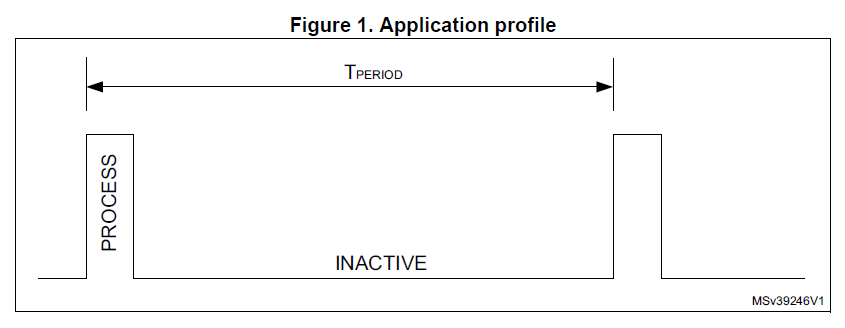
\includegraphics[scale= 0.6]{Application profile.png}
	\caption{Diagram showing a general low power operation profile for the microcontroller with two distinct phases: process and Inactive occurring over a period T.}
	\label{fig:appr}
\end{figure}

Figure \ref{fig:appr} above details a typical low power operation which can be expected from the buoy. For a typical application, we consider two main phase:

\begin{enumerate}
	\item Process phase: The system is in run mode with peripherals active at regular intervals.
	\item Inactive phase: The system is asleep untill triggered by a wake-up event (RTC) or interrupt (GPIO).
\end{enumerate}

Once the buoy has finished an active routine, the system becomes inactive between samples. The ice drift sample period was selected to be once every half an hour to provide a higher temporal resolution to characteristic the inter-sample behavior of ice floes described by \textcite{vichi2019effects} in Chapter \ref{ch:chapter2}. Therefore, once the routine is complete, the device will be inactive for tens of minutes until required. This is the inactive between sample mode and is our period of inactivity where we can place the device in the lowest possible state with very little concern for wake-up time or peripheral settings. Therefore, the following power modes were selected for each phase of the system's operation.

\begin{table}[H]
	\centering
	\caption{Power mode selection for each phase of the buoy's operational cycle. Power modes are preset by STMicroelectronics and are based on the device's architecture. A full explanation of each power mode can be found in \cite{stm32l4ref}.}
	\begin{tabular}{lll}
		\hline 
	\textbf{Phase} & \textbf{Power mode} & \textbf{Current draw}\\
		\hline
		\hline
		Process & Run mode & 1.16 mA\\
		Inactive & Standby mode & 710 nA\\
		\hline
		\hline
	\end{tabular}
	\label{tab:powmode_cycle}
\end{table}

Table \ref{tab:powmode_cycle} shows the selected power mode and the estimated current consumption of each mode \cite{stm32l4}. The run mode current was benchmarked using a Dhrystone test with a system clock of 24 MHz and code loaded from Flash. The inactive current draw was estimated with a low speed external (LSE) oscillator supplying the real time clock. 

\section{Main program design}
 
As outlined in the user requirements in Section \ref{sec:sec3_UR}, the SHARC buoy aims to increase remote sensing on both a temporal and spatial scale. Each sensor has its own sampling requirement which needs to be synchronised to the clock speed of the processor. Furthermore, the device needs to monitor and control the subsystems to ensure they are functional and opperational. Finally, subsystem power consumption needs to be carefully controlled to ensure the device opperates in a power efficient manner. The main program was designed to meet these requirements by providing a frame to sequence sensor activities. The firmware was also designed to provide time-critical execution of sensor routines to ensure that the temporal integrity of the data set was achieved. To achieve this, a state machine was selected and implemented on the STM32L4 microcontroller. \par

A state machine can be implemented to provide a high-level form of control over the system. This can be achieved by decomposing the overall function of the buoy into a series of finite states. These states are connected through a series of transitions which can be described using Boolean techniques. Through this, the buoy retains a modular structure both in firmware and in hardware which can allow for additionally sensors and functions to be implemented seamlessly.\par 

\subsection{Execution}

The goal of the buoy is to sample environmental, GPS and power data at fixed rates. $T_{sample}$ will be used to describe the period between sampling the sensor devices. Each data point will be condensed into a byte packet and stored in the external Flash chips. A decision was made to synchronise the transmission period to four samples so as to reduce the time the Iridium modem is turned in. This device consumes the most power so having it used as infrequently as possible will allow the device to conserve more power. During the transmission phase, the device will read the data packets from memory into a buffer and transmit the data. When the device exits this state, it will reset the sample count and repeat until the buoy is turned off or loses power. The buoy can therefore be broken down into a set of finite states which are shown below:

\begin{enumerate}
	\item \textbf{Initialisation state:} The device initialises the counter and verifies the sensors.
	\item \textbf{Reset state:} During this state, the sample counter is reset and the Flash chips are formated to prevent old data from corrupting the set.
	\item \textbf{Sample state:} During this state, the device actively receives data from the sensors and stores them into a packet which is then saved to a memory location.
	\item \textbf{Sleep state:} The device enters this state between samples and active states. Here, the device will remain in this state for a time $T_{sample}$. After which, the buoy will wake up.
	\item \textbf{Transmit state:} The device will load the data from memory and transfer to the Iridium modem buffer. Upon successful transmission, it will enter the reset state.
\end{enumerate}

Each state will control which routines are performed during the function and provide the system with information on the current status of the device. During run time, system information will be saved to the back up registers of the RTC. These registers will constantly be updated to show what state the buoy is in, what the last action was and what the memory status of the Flash chips is. Should the device encounter an unexpected hardware reset, the system can read the back up registers, load the last state and run as normal. A typical system run is shown in Figure \ref{fig:state_run}:

\begin{figure}[H]
	\centering
	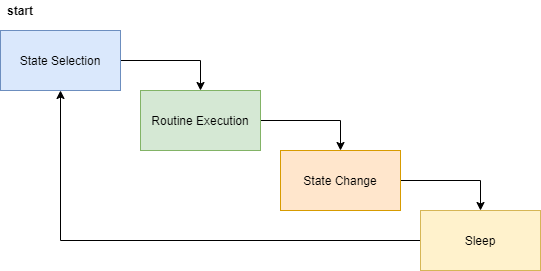
\includegraphics[scale = 0.5]{state Run.png}
	\caption{Diagram showing a typical run of the main program. The program is designed to run sequentially based on the previous completed state. The program begins from power on/wake up and reads the last known state from the RTC back up registers. Based on this state, the program will execute the corresponding routine. Finally, the program will determine the next state and write this to the back up register. If no activity is required, the device will enter low power mode.}
	\label{fig:state_run}
\end{figure}

The inputs to the state machine are:
\begin{enumerate}
	\item \textbf{C}: a 2-bit integer signifying the number of samples performed $(0 \leq N <4)$
	\item \textbf{T}: Variable that matters when the system is asleep. Signifies whether the system has been in sleep mode for a time defined by the constant value $T_{wake}$. 
\end{enumerate}
The RTC contains a wake up unit which stores this value while a counter running at 1 Hz counts in a separate register. When the counter reaches $T_{wake}$, an interrupt is generated on an internal wake up line and the device exits low power mode. \par
The system has no explicit outputs. However, the state machine is used to control which routines will be executed during the execution phase of the program. Therefore, the outputs can be considered as routines \textbf{R$_\text{x}$} as shown below:

\begin{enumerate}
	\item $R_{sample}$: Functions to initialise and sample a sensor. This routine is called for any sensor during its sample window.
	\item $R_{sleep}$ : Function to put device to sleep for a period $T_{wake}$. During this time, the device will not respond to any stimulus with, two exceptions:
		\begin{enumerate}
			\item An interrupt generated on an internal wake up line.
			\item An external interrupt generated on one of five wake up pins.
		\end{enumerate} After wake up, the device resumes functionality.
	\item $R_{gransmit}$ : Routine to initalise the Iridium modem and prepare the data for transmission. After transmission, the modem is deinitialised and put into power saving mode.
\end{enumerate}

Given the following information, the Algorithmic State Machine (ASM) chart is derived and shown in Figure \ref{fig:ASM_chart}.

\begin{figure}[H]
	\centering
	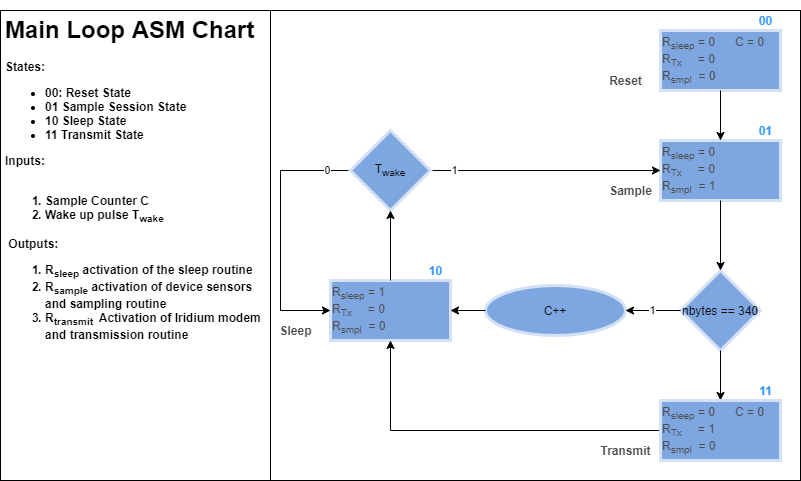
\includegraphics[width= \textwidth]{Main Loop ASM Chart.png}
	\caption{ASM chart for the proposed state machine to run on the processor showing entry/exit conditions and functions to be run during states.}
	\label{fig:ASM_chart}
\end{figure}

Figure \ref{fig:ASM_chart} shows an abstract representation of the logical flow of the program. A typical run from the system will have the buoy initialised and calibrated before entering the main loop where it will alternate between active sampling and inactive sleep mode until enough data have been collected to transmit. This allows the Iridium modem to only be turned on when needed thereby significantly conserving energy while allowing for the system to sample as much as possible. The variable $T_{wake}$ is user defined and sets the sample rate of the system. As mentioned previously, the interval for measuring ice drift was set to 30 minutes with data transmitted on the fourth cycle.

The RTC periodic wake up unit is used as a counter in deep sleep mode. This is a 16-bit down-counting Auto Reload Register \textit{(ARR)} that generates an interrupt on an internal wake up line when the system has slept for a length of time \textit{T} as defined by the user. In addition, the sample counter gets reset after every transmission state and when the buoy enters a reset state. The number of samples before transmission was chosen to be four. Since the Iridium transmission buffer is 340 bytes long and the RockBLOCK data service charges \pounds0.14\footnote{Source: \url{https://www.rock7.com/products/rockblock-9603-compact-plug-play-satellite-transmitter} as of March 2021} per 50 bytes, the goal is to transmit as much data that would fit into the buffer as possible. Too frequent transmissions incur a high data cost but result in data integrity. Too few transmissions can result in lost sample points if a transmission is not received. As a result, transmissions will occur every 2 hours with an expected total of 12 transmissions each day. The reason for this will be discussed in Section \ref{sec:dm}.

\subsection{Asynchronous behaviour}
\label{subsec:ch5_asynch}
Asynchronous behavior describes all functionality that occurs outside of the main loop. This can come from interrupts or external events which causes the system to exit the main loop regardless of state. For this version of the buoy, asynchronous functionality was considered for the Iridium modem to allow the device to receive messages. This would allow for users to interact with the device and receive data outside the scheduled transmission period. Further asynchronous functionality was added for the inertial measurement unit. This would allow for easier data flow from the sensor (see section \ref{sec:data_flow}) and allow for event-based sampling. The following are sources of asynchronous behavior:

\begin{enumerate}
	\item Interrupts
	\begin{enumerate}
		\item Iridium messages received (ring alert)
		\item IMU event detection (ice floe collision/free-fall detection)
	\end{enumerate}
	\item Events
	\begin{enumerate}
		\item Low power detection
		\item Brown out detection
		\item Software resets
		\item Watch dog resets
	\end{enumerate}
\end{enumerate}

These events take precedence over the main loop function. A full description of events, interrupts, and the protocols for handling them are shown in Tables \ref{tab:Int_desc_RI} to \ref{tab:Ev_desc_SWR} in Appendix \ref{sec:evt}. The figure below shows how the event handling procedure is sequenced in the main program:

\begin{figure}[H]
	\centering
	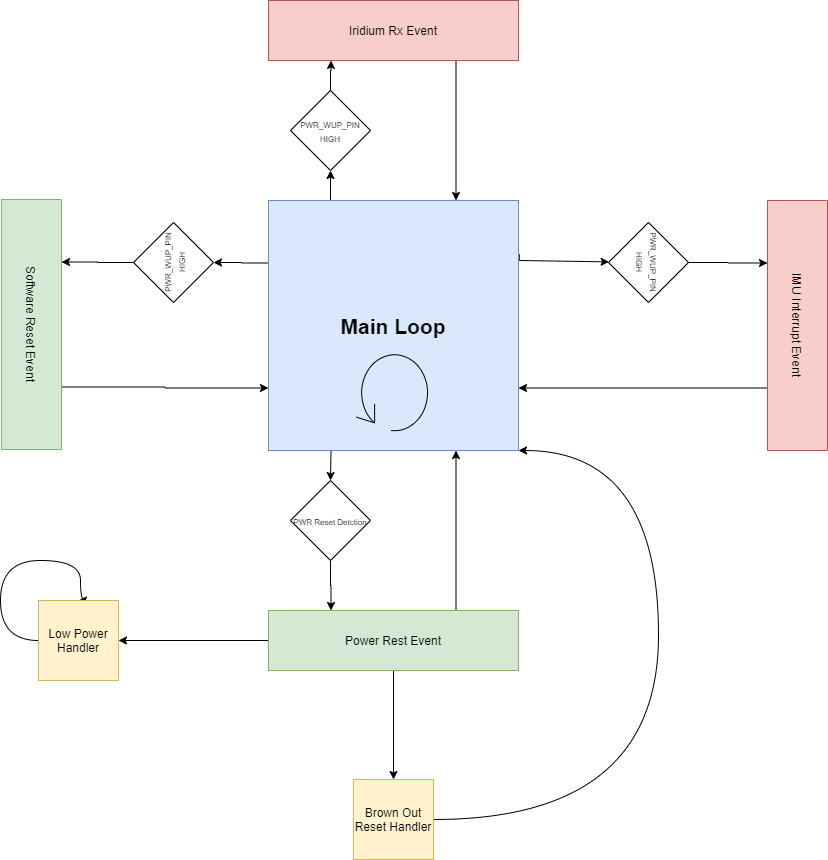
\includegraphics[width = \textwidth]{Asynchronous State diagram.png}
	\caption{Application diagram with event and interrupt sequencing.}
	\label{fig:main software}
\end{figure}

States are represented by unsigned 8-bit integers on the system and are represented in Table \ref{tab:state_bit}.

\begin{table}[H]
	\centering
	\caption{Numerical and 8-bit unsigned integer representation of the synchronous states on the STM32L4 microcontroller.}
	\label{tab:state_bit}
	\setlength{\textwidth}{5pt}
	\begin{tabular}{clc}
		\hline
		\textbf{State number} & \textbf{State name} & \textbf{8-bit representation}\\
		\hline
		\hline
		0 &Reset 	& 	0b0000 0000\\

		1 &Sample 	& 	0b0000 0001\\ 
	
		2 &Sleep 	& 	0b0000 0010\\
	
		3 &Transmit & 	0b0000 0011\\
		\hline
		\hline
	\end{tabular}
\end{table}

The backup are used to store state information while the buoy is in deep sleep. These registers are located at the memory addresses: 0x40002850 to 0x400028CC in the STM32L4 memory map \cite{stm32l4ref}. These registers keep data even when the device is in low power mode or a software reset has occurred therefore making them the perfect storage location. The state variable holds the value of the current state of the buoy. This variable is stored in two locations: When the system is in run mode, the value is stored in the global variable \textit{Current\_State}. When the device is in a deep sleep state, the variable is stored in the RTC back up registers at byte 0 of back up Register 0. Upon wake up, the value is loaded from the register and placed in the global variable.

The main loop follows a sequential state transition as described in Figure \ref{fig:main software}. To achieve this, at the start of each loop, the program reads the value stored in the state variable. This determines what the previous state was. Based on this value, the new state is determined and stored in the state variable. This process is shown in the figure below.

\begin{figure}[H]
	\centering
	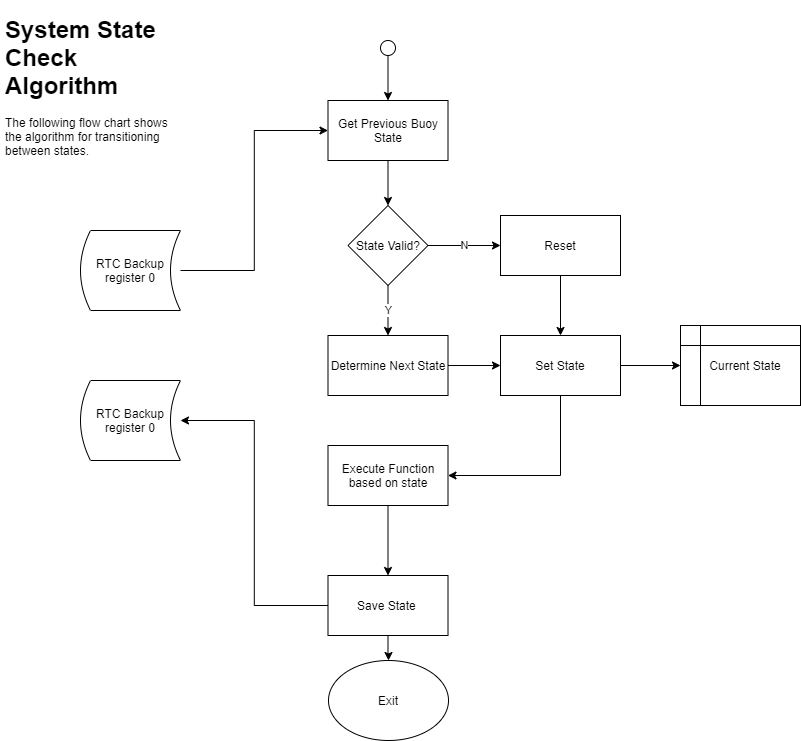
\includegraphics[width=\textwidth]{State Check Algorithm.png}
	\caption{Flow chart for the state-check algorithm}
	\label{fig:state_check}
\end{figure}

Figure \ref{fig:state_check} above shows the algorithm for selecting and transitioning between states. This algorithm allows for states to be linked in any order and, most importantly, separates the state selection from the state function. By separating these two concepts, a more modular framework is created. This allows for the addition of more states and transitions without modifying the routines that are currently in place. This allows for device functions to be turned on and off as desired without drastic changes to the firmware.

Finally, asynchronous states take a higher precedence over the main loop states and are checked before the state check shown above. The order of precedence is shown in the table below:
\begin{table}[H]
	\centering
	\caption{Table showing the types of states that the system checks for ordered by priority with 1 being the highest priority and 3 being the lowest.}
	\begin{tabular}{lc}
		\hline
		Name & Priority \\
		\hline
		\hline
		Power event & 1 \\

		Asynchronous interrupt & 2 \\
		\hline
		Sequential state & 3 \\
		\hline
		\hline
	\end{tabular}
	
	\label{tab:state_prio}
\end{table}

Power events generate a system reset and raise a flag in the \textit{PWR} status register. When the flag is set, the program enters the handler and, if the event is non-fatal, returns to the main loop. The following flow chart shows an example of such a case for a brown out event.

\begin{figure}[H]
	\centering
	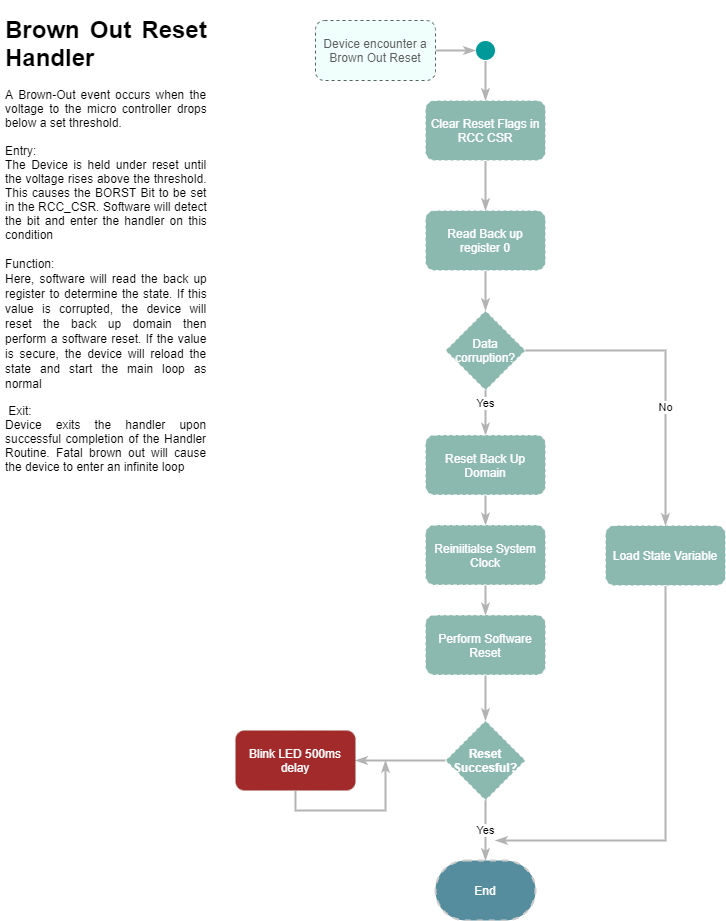
\includegraphics[width=\textwidth]{Brown Out Reset Handler Flow Chart.png}
	\caption{Diagram showing the algorithm for brown out event recovery and handling.}
	\label{fig:evt_handle}
\end{figure}

Some sensors have interrupt pins and can be configured to trigger upon detection of a specific event. When this happens, the sensor will send a digital high on the interrupt pin. On the processor side, a hardware interrupt is generated and the software handles the interrupt. An example of such a procedure is shown in Figure \ref{fig:int_handle}.

\begin{figure}[H]
	\centering
	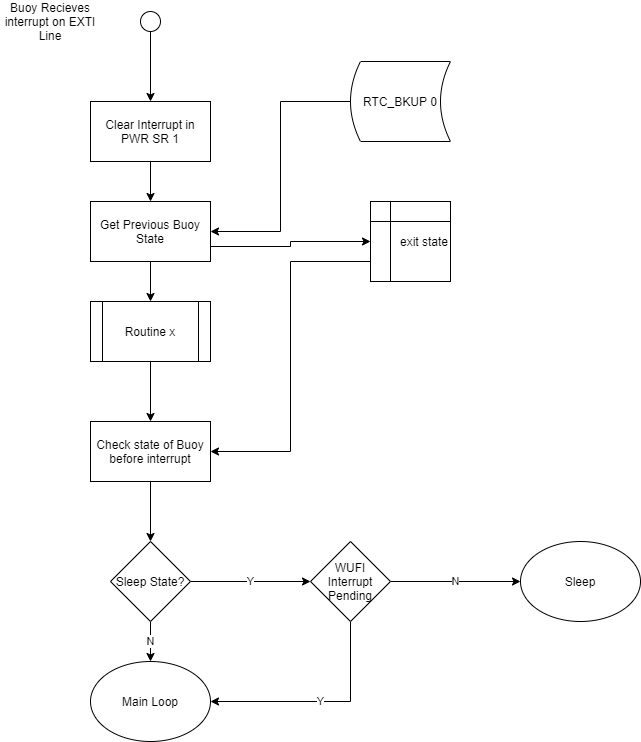
\includegraphics[width=\textwidth]{Asynchronous State flow chart.png}
	\caption{Diagram showing the algorithm for handling an external interrupt from a Wake Up pin connected to one of the modules}
	\label{fig:int_handle}
\end{figure}

By connecting these pins to external wake up pins, the buoy is capable of event detection in deep sleep mode. If an event is detected while in deep sleep, the interrupt causes the buoy to wake up and resume from the beginning. No interrupt handler is entered at this point. A flag is set in the \textit{PWR\_SR} at the position of the wake-up pin it detected. The buoy will enter the asynchronous state depending on which flag is set and will execute the routine associated with it. When the buoy wakes up from an internal wake up timer, the pins are reconfigured into \textit{GPIO EXTI} mode which allows the buoy to receive interrupts when active. It was found that by keeping these configured as wake up pins during run time, the system reset when an interrupt was detected. Therefore, strict measures were taken to ensure that the pins were reconfigured at every point in the program that is entered when the device wakes up from deep sleep.

\subsection{Subsystem execution}

When a module is is being used at any point in the program. The microcontroller will execute an initialise routine. This will enable any required peripherals for communication with the subsystem. This function will be called before every sample period in case the system encounters a power surge or an unexpected reset. Additionally, placing the microcontroller in deep sleep mode results in the registers being reset upon wake up. The initialisation routine is specific to each microcontroller and includes the following:

\begin{enumerate}
	\item High level communication peripheral configuration.
	\item Low level pin configuration
	\item Sensor verification function
	\item Sensor configuration function
	\item Return status
\end{enumerate}

The outcome of the initialisation routine is evaluated based on a return status from the function. This ensured that the status of the device was known at all times. If the device was offline, the program would either retry to connect to the module or continue execution without it. This ensured that the program was robust enough to deal with hardware failures as experienced by \textcite{doble2017robust} and \textcite{rabault2018investigation}. Items 1 to 3 are included to configure the subsystem to adhere to the functional requirements in Table \ref{tab:sys_specs}. Sensor verification functions are included to satisfy acceptance tests AT001 and provide evaluations for acceptance tests AT002 and AT004. These functions also allow the program to continue execution if a sensor becomes corrupted or a communication channel becomes non-responsive. The initialisation function is designed handle fail modes by evaluating the system's failure return type and responding in accordance with the protocols outlines in acceptance test AT002. initialisation routines for each subsystem is provided in Appendix \ref{fig:Init_diagram_gps} to \ref{fig:Init_diagram_mpu}.

If the initialisation was successful, the program will continue using the module in the firmware. Should a failure occur, the system will attempt to reconnect with the device a predefined number of times. In case of a critical failure, the system will acknowledge that it can no longer use the device and will continue the main firmware without it. The resulting behaviour is shown in Table \ref{tab:exe_subsy_Failiure}.

\begin{table}[H]
	\centering
	\caption{Table Showing the device behavior in case of a critical failure in one or more of the subsystems. Critical failures are defined in AT006 (Table \ref{tab:AT006}) testing protocol.}
	\setlength{\extrarowheight}{5pt}
	\resizebox{\textwidth}{!}{
	\begin{tabular}{lll}
		\hline
		\textbf{Device failure case} & \textbf{Impact} & \textbf{Result}\\
		\hline
		\hline
		Iridium & Critical & No data will be transmitted from the buoy. \\
		\hline
		Flash chips & Critical & Data will be lost when power is reset. \\
		\hline
		GPS & High & Critical GPS data will not be captured. \\
		\hline
		MPU6050 & High & Unable to measure crticial accelerometer and gyroscope data. \\
		\hline
		Environment Sensor & Medium & Environmental data will not be captured. \\
		\hline
		Power monitor & Low & Current and voltage measurements will not be captured. \\
		\hline
		\hline
	\end{tabular}}
	\label{tab:exe_subsy_Failiure}
\end{table}

In conclusion, defensive functions were added to ensure the firmware interface with the hardware sensors is robust and recoverable in case of hardware failure. 
\section{Data management}
\label{sec:dm}
A critical consideration for the system is the flow of data and memory management. The Flash chips provide a solution for permanent storage however, it is critical that data integrity be maintained. Some form of data organisation must be implemented for intelligent retrieval/storage of data in a meaningful way. In addition, the system requires some form of back up should the device be unable to connect to the Flash chips. This section outlines the data organisation and storage methods implemented in the firmware to ensure efficient retrieval and storage of data. \par 

The Flash chips used are Adesto TEchnologies AT45DB641E SPI serial Flash chips. Each chip can hold up to 64 Mbit of data. Data can be read/written at speeds of up to 85 MHz or 15 MHz in low power mode. The device is low power with high data retention requiring a supply voltage of 1.7 V to 3.6 V and draws a maximum of 11 mA in active read mode thereby making it one of the lowest power consumption components in the system. In addition, the device comes with two 256 byte buffers that can store data while a read/write operation is taking place. Memory is organised into sectors (2 to 256 KBs long), blocks (2 KB long) and pages (256 bytes) with write, read and erase options at each level. In this section, the data requirements from each sensor are listed. The optimal storage strategy is to convert the measurements into binary data and store as an array of bytes at known locations in an array. \par 

\subsection{Debugging}

As discussed in Chapter \ref{ch:ch3}, a key user requirement for developing the SHARC buoy is ensuring the design is robust. This means that device must be capable of providing feedback of system and subsystem states either to the users or between the different firmware layers. Furthermore, from the stakeholders in Table \ref{tab:stake}, users of the buoy may not necessarily be involved in the design and development phases and therefore must rely on other methods to understand whether the device has deployed successfully or whether the system is online. To achieve this error checking methods were implemented in all algorithms to ensure that functions executed as predicted and current status of the buoy was known at all times. These subsections discusses the debugging methods both internal and external to the buoy.

\subsubsection{Internal debugging}

Internal debugging was achieved by ensuring that each layer of the system had defensive measures built into the algorithms. For example, on the device driver layer, the communication algorithms had built in timeouts to prevent the system from freezing while waiting for input. These functions returned error codes to the higher layers when called. On this level, different errors were accounted for by creating an enumeration of error types as shown in Figure \ref{fig:errorcode}.

\begin{figure}[H]
	
	\begin{lstlisting}
typedef enum{
	GPS_Init_OK = 1,
	GPS_Init_Ack_Error = 2,
	GPS_Init_Baud_Config_Error = 3,
	GPS_Init_MSG_Config_Error = 4,
	GPS_Init_Ack_Tx_Error = 5,
	GPS_Init_Periph_Config_Error = 6,
	GPS_Init_Offline_Error = 7
}GPS_Init_msg_t;
		
	\end{lstlisting}
	\caption{ Example of an enumeration of possible error sources for a peripheral library function. Each error code is a numeric value which is returned when a specific error condition is encountered thereby providing feedback to higher levels.}
	\label{fig:errorcode}
\end{figure}


 On the device peripheral level, if an error code was returned, the routine that called the functions would evaluate the error code and act accordingly. If the failure was critical, this feedback would be provided to the main program which would then break out of the routine and continue with the primary loop.
\subsubsection{External debugging}

Progress was monitored via visual indication. Having a visual indicator ensured that the buoy progress was constantly known without needing to interfere with the program execution or peak into the code. This allows the user to understand how the buoy operates without needing the firmware or references to the firmware. This was achieved by using a green LED onboard the STMicroelectronics Nucleo-L476RG development board. The green LED was programmed to execute Flashing sequences at various points in the code to signify information such as sensors were online or a routine was in progress. This allowed for remote debugging of the platform. However, this method does not offer any detailed information about the status of the buoy. \par

To provide more information, a free UART port was programmed to output status information to a serial terminal. This allows a user to view more detail regarding the current state the buoy is in, the state of the sensors and the incoming data. However, this technique requires a constant connection and is not suitable for deployment.
\subsection{Drift data acquisition}

This section describes how data are acquired from the sensors to form an ice drift measurement packet. Readings are taken from the GPS and environmental sensor with the power monitor being sampled to provide an update on the buoys performance.\par 

\subsubsection{Overview of drift data}

The GPS is sampled four times over a given interval at each sample point, the following data are recorded:


\begin{enumerate}
	\item Time and date information
	\item Geographical coordinates
	\item Dilution of precision
	\item Diagnostic information
\end{enumerate}

%Discuss UART
By default, the u-blox NEO-7M and NEO-M9N receivers uses the National Marine Electronic Standards (NMEA)\footnote{Information about NMEA messaging on the u-blox Neo GPS is taken from \cite{UBLOX_M9N_INTERFACE}} to format data. These have the following format:

\begin{table}[H]
	\centering
	\caption{ Breakdown of a typical NMEA message string with fields indicating start/stop sequences and character information.}
	\begin{tabular}{|c|c|c|c|c|c|}
		\hline
		\$  & \multicolumn{2}{|c|}{Address} & Data Field & checksum & End Sequence\\
		\hline
		\multicolumn{1}{c|}{} & TT & SSS &\multicolumn{3}{c}{} \\
		\cline{2-3}
	\end{tabular}
	\label{tab:GPS_data_format}
\end{table}
\begin{itemize}
	\item \$ - Character denoting the start of the sequence.
	\item Address - This is a 5 byte character sequence that is used to provide information on the talker ID (TT) and the the type of information in the payload (SSS).
	\item Data field - Data in this field is formatted as a character sequence separated by commas. This field holds the payload specified by the payload information characters in the address field.
	\item Checksum - Sequence of characters denoted by a "*" and followed by two bytes in ASCII hexadecimal format. These values are calculated by performing an XOR operation on all the bytes between the "\$" and "*" characters.
	\item End Sequence - 0x0D, 0x0A denotes the end of the NMEA message.
\end{itemize}

NMEA messages are standardised in the format given in Table \ref{tab:GPS_data_format}. However, each NMEA message holds different information. Therefore, the incoming message strings can have different lengths depending on the messages that have been enabled. To accommodate this in the firmware, a data streaming channel needs to be set up to allow for an unknown number of bytes to be transferred through serial communication in an efficent way. Furthermore, to ensure that the required GPS drift data were obtained, Tables \ref{tab:NMEA_ZDA} to \ref{tab:NMEA_GLL} show the NMEA messages that were selected and the data as well as the format of each of the fields.

\begin{table}[H]
	\centering
	\caption{Description of ZDA message string showing variables, description and how the example datum 5th September 2002 08:27:10 am is stored.}
	\setlength{\extrarowheight}{5pt}
	\tiny
	\begin{tabular}{lll}
		\hline
		\hline
		\multicolumn{3}{c}{\textbf{ZDA - time and date}}\\
		\hline
		\hline
		\textbf{Description} & \multicolumn{2}{l}{Datum information in UTC representaion}\\
		\hline
		\textbf{Variable name} & \textbf{Format}& \textbf{Example} \\
		\hline
		\hline
		UTC time & hhmmss.ss & 082710.00 - 08:27:10 am\\
		
		UTC day & dd & 05 - 5th \\
		
		UTC month & mm & 09 - September\\
		
		UTC year & yyyy & 2002 \\
		
		Time zone hours & hh & 00 (+00)\\
		
		Time zone minutes & mm & 00 (+00)\\
		\hline
		\hline
	\end{tabular}
	\label{tab:NMEA_ZDA}
\end{table}

\begin{table}[H]
	\centering
	\caption{Description of GSA message string showing variables, description of parameters and how the variables are stored.}
	\tiny
		\setlength{\extrarowheight}{5pt}
	\begin{tabular}{lll}
		\hline
		\hline
		\multicolumn{3}{c}{\textbf{GSA - fix diagnostic}}\\
		\hline
		\textbf{Description:} & \multicolumn{2}{l}{ DOP, number of satelites and fix type}\\
		\hline
		\hline
		\textbf{Variable name} & \textbf{Format}& \textbf{Example} \\
		
		Opperation mode & A/M & A - Automatic\\
		
		Navigation mode & Number (1-3) & 1 - No fix \\
		
		Satelite ID & Number & 29 - Satelite number \\
		
		Direction & C & E - East \\
		
		PDOP & Float & 1.91 \\
		
		HDOP & Float & 1.18 \\
		
		VDOP & Float & 1.14 \\
		\hline
		\hline
	\end{tabular}
	
	\label{tab:NMEA_GSA}
\end{table}

\begin{table}[H]
	\centering
	\caption{Description of GLL message string showing variables, description and how a set of coordinates e.g. (47$\degree$17.11364'N, 8$\degree$ 33.91565' ) is stored.}
	\setlength{\extrarowheight}{5pt}
	\tiny
	\begin{tabular}{lll}
		\hline
		\hline
		\multicolumn{3}{c}{\textbf{GLL - Geographic coordinates and fix}}\\
		\hline
		\textbf{Description:} & \multicolumn{2}{l}{ latitude and longitude with positional fix information.}\\
		\hline
		\hline
		\textbf{Variable name} & \textbf{Format}& \textbf{Example} \\
		
		Latitude & ddmm.mmmmm & 4717.11364 - 47$\degree$17.11364'\\
		
		Direction & C & N - North \\
		
		Longitude &dddmm.mmmmm & 00833.91565 - 8$\degree$ 33.91565' \\
		
		Direction & C & E - East \\
		
		Fix status & A & A - Valid\\
		\hline
		\hline
	\end{tabular}
	
	\label{tab:NMEA_GLL}
\end{table}

\subsubsection{GPS sampling strategy}
\label{subsec:CH5_gpsss}

The u-blox NEO-7M/NEO-M9N module continuously outputs data at a fixed rate of 1 Hz \cite{UBLOX_M9N_INTERFACE} through Universal Synchronous/Asynchronous Transmission. The device comes preset with not all NMEA messages active. The messages were enabled by writing to the \textit{CFG-MSGOUT} register. This was achieved by transmitting a customised configuration string to the u-blox module. If successful, the receiver will return an acknowledgment message.\par 

Then a UART data stream was created to read the incoming messages. To achieve this, one could poll the receiver register for the byte information. However this method requires additional processing power which increases the power consumption. Additionally, constantly polling the register can result in data being overwritten if it is not read fast enough. The STM32L4 microcontroller contains a direct memory access (DMA) controller \cite{stm32l4ref} which allows for data to be streamed directly from a peripheral to a specified address in memory. This method was preferred as it allows for data to be read from the sensor without constraining processor resources. \par 

Reading data through a DMA channel requires knowledge of the number of bytes being received. However, as mentioned previously, this value is not known. Therefore, a solution was to manually turn off the DMA stream when no data were received for a certain length of time (i.e. an idle line condition). This was achieved by setting up a timer channel in input capture mode on the receiver line in slave reset mode while another channel was configured in output compare mode. In this register, the expected idle period was stored. Incoming data would reset the counter in the input capture channel. If the counter reached the value in the output compare channel, an interrupt was generated which signaled the DMA to stop the transfer. The number of bytes transferred was stored, the DMA was reset and the data were stored. \par 

As an additional precaution, data from the peripheral DMA stream was backed up to protect the data against accidental deletion or corruption. This was done by using another DMA stream set from the current data memory address to another data buffer via memory to memory DMA stream triggered on completion of the peripheral to memory DMA stream. This streaming technique formed a UART DMA circular buffer with a slave reset trigger.\par 

Then, message parsers were written to extract the information from the message strings and convert them into a binary representation. These message parsers contain a check for validity. This algorithm first checks that the data follows the correct NMEA formatting as shown in Table \ref{tab:GPS_data_format}. Then it analyses the address to ensure that the talker ID and message-ID are valid. Finally, it calculates the two-byte checksum by performing an exclusive OR on all the bytes in the data field and compares them to the checksum bytes that were sent with the packets. Message parsers were written for GLL, GSA and ZDA messages and were called based on the return status of the validity check. Table \ref{tab:GPS_Data} shows the memory allocation for each variable. 

\begin{table}[H]
	\centering
	\caption{Data collected from the GPS in a single sample session. Square brackets denote a numbered sequence of like variable types.}
	\small
	\setlength{\extrarowheight}{5pt}
	\tiny
	\begin{tabular}{llc}
		\hline
		\textbf{Variable name} & \textbf{Variable type} & \textbf{Size [bytes]} \\
		\hline
		\hline
		Epoch time & Unsigned 32-bit integer & 4 \\
		Latitude & Signed 32-bit float & 4 \\
		Longitude & Signed 32-bit float & 4 \\
		HDOP & Unsigned 8-bit integer[2] & 2\\
		VDOP & Unsigned 8-bit integer[2] & 2\\
		PDOP & Unsigned 8-bit integer[2] & 2\\
		Diagnostic information & Unsigned 8-bit integer & 1 \\
		\hline
		\hline
		\cline{3-3}
		\multicolumn{2}{r}{Total: } & \multicolumn{1}{c}{19}\\
		\cline{3-3}
		
	\end{tabular}
	\label{tab:GPS_Data}
\end{table}

Time and date information were combined and converted into Unix epoch time. This represents the number of seconds that have elapsed since a defined epoch (1 January 1970) which allows for a single, 4-byte variable to represent both time and date. Geographic coordinates have been converted into signed 32-bit floats with the sign representing the direction of the coordinate. The coordinates were then split into an array of 4 unsigned 8-bit integers and recombined using IEEE-754 as a standard. The dilution of precision represents a value between 0 and 99.99 therefore, the optimal storage solution is to allocate a byte for the digit and a byte for the precision. Finally, diagnostic information includes the fix type and the number of satellites. A maximum of 15 satellites can be used to determine a position. These data can be stored in the lower four bits of a single 8-bit integer. The fix type is a number from 1 to 3 therefore only taking up 2 bits of a byte.\par 


\subsection{Environmental data acquisition}
The BMP280 contains two onboard Analog to Digital Converters (ADCs) which are used to convert the pressure and temperature measurements into unsigned 8-bit values. Each measurement is stored as three unsigned 8-bit integers in three registers and must be read sequentially to get the full measurement. Once retrieved, the data must be combined into a 24-bit word which results in the raw, uncompensated ADC value. The BMP280 also contains a configurable infinite impulse response (IIR) filter as well as configurable oversampling parameters for the pressure and temperature measurement. Data are read through an SPI communication interface into the microcontroller by performing a burst read of 6 bytes. To compensate for the mechanical effects of each sensing element, the device comes preloaded with a set of compensation parameters for the temperature and pressure reading \cite{BMP280_Datasheet}. The compensation algorithms are shown in Appendix \ref{fig:bmp_code_comp_P} and \ref{fig:bmp_code_comp_T}. The output of the compensation algorithm are shown in Table \ref{tab:BMP_output}.

\begin{table}[H]
	\centering
	\caption{Description of output values from BMP280 post processing.}
	\setlength{\extrarowheight}{5pt}
	\tiny
	\begin{tabular}{llllc}
		\hline
		\textbf{Name }& \textbf{Type} &\textbf{Format} & \textbf{Example} & \textbf{Total [bytes]}  \\
		\hline
		\hline
		Temperature & Signed 32-bit integer & CCcc$\degree$ C & 2508 to 25.08$\degree$ C & 4\\
		Pressure & Signed 32-bit integer & PPPppp kPa & 100653 - 100.653 kPa & 4\\
		\hline
		\hline
		\multicolumn{4}{r}{\textbf{Total}} & \multicolumn{1}{c}{8}\\
		\cline{5-5}
		\cline{5-5}
	\end{tabular}
	
	\label{tab:BMP_output}
\end{table}

\subsection{Power data acquisition}

The INA219 samples current across a shunt resistor of a known value. In this application, the shunt resistor provided is 0.1 $\Omega$. The device also samples the voltage across the shunt resistor through a programmable gain amplifier (PGA) before being sampled by an ADC. The sensor stores data as 16-bit integers. Negative values are stored in two's complement format. Data are transferred via I$^2$C to the microcontroller after the conversions have taken place. The sensor measures both shunt and bus voltage which, when combined, provide an estimate of the voltage across a load. The output resolution can be programmed as either 9-bit, 10-bit or 12-bit. When the device is initialised, it needs to be calibrated. A calibration routine was developed for the device based on the algorithm recommended by \textcite{INA219}. The bus range voltage was chosen as 16 V with a maximum expected current of 1.2 A (two times the expected peak current draw) to be safe. The output of the calibration procedure is a 16-bit word that is written to the calibration register. The algorithm used to calibrate the sensor for the SHARC Buoy application is outlined in Appendix \ref{fig:INA_Calib} with the following parameters:
\begin{table}[H]
	\centering
	\caption{ Description of parameters used to calibrate the INA219 current sensor.}
	\setlength{\extrarowheight}{5pt}
	\tiny
	\begin{tabular}{l c}
		\hline
		\hline
		\textbf{Maximum bus voltage}& 16 V \\
	
		\textbf{Maximum expected current} & 1.2 A \\
	
		\textbf{Shunt resistor} & 0.1 $\Omega$ \\
	
		\textbf{Shunt voltage range} & $\pm$160 mV\\
		\hline
		\hline
	\end{tabular}
	
	\label{tab:INA_Calib}
\end{table}

The sensor calculates the power consumption as a signed 16-bit number by multiplying the bus voltage ADC reading with the current ADC reading and placing it in the power register. The microcontroller performs a burst read of the bus voltage, shunt voltage, current and power register and stores the values as signed 16-bit integers. The bus voltage register reserves the first three bits of the register for signal flags. Therefore, the bus voltage reading must be shifted by three bits to the right to remove them. Finally, the power reading is multiplied by the LSB step size size calculated in the calibration routine which results in a signed 16-bit integer representation of the power in milliwatts (mW). The data requirements are shown in Table \ref{tab:INA_Output}

\begin{table}[H]
	\centering
	\caption{Description of output values from INA219 current sensor.}
	\setlength{\extrarowheight}{5pt}
	\resizebox{\textwidth}{!}{
	\begin{tabular}{llllc}
		\hline
		\textbf{Name }& \textbf{Type} &\textbf{Format} & \textbf{Example} & \textbf{Total [bytes]} \\
		\hline
		\hline
		Shunt voltage & Signed 16-bit integer & vvvmm & 18049 to 180.49 mV & 2 \\

		Bus voltage & Signed 16-bit integer & VVvvv & 08025 to 8.025 V & 2 \\

		Current & Signed 16-bit integer & IIIii & 51234 to 519.23 mA & 2 \\
	
		Power & Signed 16-bit integer & PPPPpp & 28130 to 2813.00 mW & 2 \\
		\hline
		\hline
		\multicolumn{4}{r}{\textbf{Total}} & \multicolumn{1}{c}{8}\\
		\cline{5-5}
		\cline{5-5}
	\end{tabular}}
	
	\label{tab:INA_Output}
\end{table}


\subsection{Total ice drift data}
Table \ref{tab:total_data} below shows the total ice drift data collected from a single sample point.

\begin{table}[H]
	\caption{Total drift data collected during a single sample point.}
	\setlength{\extrarowheight}{5pt}
	\tiny
	\centering
	\begin{tabular}{lc}
		\hline
		\textbf{Device name}  & \textbf{Total data (bytes)}\\
		\hline
		\hline
		GPS & 19 \\

		Environmental Sensor & 8 \\

		Power Monitor & 8\\
		\hline
		\hline
		\multicolumn{1}{r}{\textbf{Total}} & \multicolumn{1}{c}{35}\\
		\cline{2-2}
		\cline{2-2}
	\end{tabular}
	\label{tab:total_data}
\end{table}

Table \ref{tab:total_data} shows that 35 bytes of data are collected during a single sample session if all the sensors (excluding IMU) are sampled concurrently. Since the device has four Flash chips each with a capacity of 8 MB, the device contains 32 MB of permanent storage space. This is enough memory to store 914285 full packets of drift data. At 30 minute intervals, this is enough to store 152.19 years worth of drift data. 
\subsection{Wave measurement data}

This section describes how data are acquired for waves in ice measurements. The inertial measurement unit (IMU) provides 3 axes of acceleration and 3 axes of angular velocity which are the components used to estimate the significant wave height, dominant wave frequency as well as the spectra and co-spectra over the sample period. IMU sampling occurs after the fourth drift measurement is taken during the buoy opperational cycle. The sample frequency was chosen to be 5 Hz to satisfy the Nyquist sampling criteria.\par 

\subsubsection{IMU sampling strategy}

The MPU6050 IMU is a micro electrical-mechanical system (MEM). The device measures the inertial axis reading which is then digitised using a 16-bit ADC for each axis of the accelerometer and gyroscope. Communication is performed using I$^2$C where the pin AD0 is used to set the I$^2$C address. In addition, the device is fully configurable allowing for programmable ADC full scale resolutions and sample rates. The device also contains an on-board digital low pass filter, the bandwidth of which can be programmed through the \textit{CONFIG} register.\par 

The MPU6050 is an 8-bit device. Measurements from the ADC are split into 8-bit bytes and stored across 2 registers (one for the most significant byte, and one for the least significant byte). A burst read operation is performed to retrieve the data in the register. The two bytes are combined and stored as a signed 16-bit integer. This value is then multiplied by a sensitivity factor which results in a float representing either the acceleration or the angular velocity. The sensitivity factor is determined based on the selected full scale range of the accelerometer and gyroscope. Table \ref{tab:IMU_data_outl} gives a breakdown of a single sample of IMU data.

\begin{table}[H]
	\centering
	\caption{Description of output values from the MPU6050 IMU showing variable name, size and significance.}
	\setlength{\extrarowheight}{5pt}
	\small
	\begin{tabular}{llc}
		\hline
		\textbf{Name} & \textbf{Type} &\textbf{Total [bytes]} \\
		\hline
		\hline
		X-axis acceleration & Signed 16-bit integer & 2\\

		Y-axis acceleration & Signed 16-bit integer & 2\\

		Z-axis acceleration & Signed 16-bit integer & 2\\

		X-axis angular velocity & Signed 16-bit integer & 2\\

		Y-axis angular velocity & Signed 16-bit integer & 2\\
		Z-axis angular velocity & Signed 16-bit integer & 2\\
		\hline
		\hline
		\multicolumn{2}{r}{\textbf{Total}} &\multicolumn{1}{c}{12}\\
		\cline{3-3}
		\cline{3-3}
	\end{tabular}
	
	\label{tab:IMU_data_outl}
\end{table}

From our user requirements the sample period for collecting wave data are a minimum of 15 minutes. Average ocean wave sample periods are recorded at 20 minutes sometimes even as high as 30 mins for significant wave height. The dominant wave frequency occurs at about 1 Hz. Sampling at 2 Hz \cite{kohout2015device} is a bare minimum. However, 5 Hz is recommended. 

\begin{table}[H]
	\centering
	\caption{Parameters of the IMU and their configured value for this application.}
	\setlength{\extrarowheight}{5pt}
	\small
	\label{tab:IMU_param}
	\begin{tabular}{ll}
		\hline
		\hline
		\textbf{Sample period [minutes]}  & 20 \\

		\textbf{Sample frequency [Hz]} & 5 \\

		\textbf{Accelerometer full scale range [g]} & $\pm$ 2\\ 

		\textbf{Gyroscope full scale range [$\degree s^{-1}$]} & $\pm$ 500\\

		\textbf{Digital low pass filter bandwidth [Hz]} & 92\\ 
		\hline
		\hline
	\end{tabular}

\end{table}

Finally, the total data accumulated over the required sample period is shown in Table \ref{tab:IMU_data_total}.

\begin{table}[H]
	\centering
	\caption{Breakdown of data accumulated from the IMU with the sample parameters mentioned in Table \ref{tab:IMU_param}.}
	\setlength{\extrarowheight}{5pt}
	\begin{tabular}{ll}
		\hline
		\hline
		\textbf{Sample frequency [Hz] }  & 5\\
		\hline
		\textbf{Sample period [s]}    & 1200\\
		\hline
		\textbf{Number of samples}  & 6000 \\ 
		\hline
		\textbf{Bytes per sample}   & 12 \\
		\hline
		\hline
		\multicolumn{1}{r}{\textbf{Total}} & \multicolumn{1}{l}{72000 bytes}\\
		\cline{2-2}
	\end{tabular}
	
	\label{tab:IMU_data_total}
\end{table}

Therefore, a total of 72 KB is collected from each session. With the current memory configuration. A single sample can occupy 0.9\% of a single Flash chip. With four 8 MB Flash chips, The buoy can record 444 raw IMU datasets. If recorded every 2 hours, this amounts to 37 days worth of data. However, due to the low bandwidth of the Iridium modem, IMU data would need to be split into packets of 340 bytes. This would require 212 transmissions to deliver a single set of data. This is not advisable due to the high current consumption of the modem as well as the long transmission times. To send all data, advanced compression techniques or a robust wave data processing algorithm needs to be implemented which falls outside the scope of this project. For testing purposes, as a proof of concept, the IMU sample period was reduced to 5.6 seconds which resulted in 28 samples or 336 bytes of data.

\subsection{Timing requirements}
\label{subsec:ch5_timing}


Table \ref{tab:sensor_timing} below shows the timing requirements for each sensor.

\begin{table}[H]
	\centering
	\caption{Timing requirements for each sensor showing the interval between samples and the number of samples collected during each session.}
	\label{tab:sensor_timing}
	\setlength{\extrarowheight}{5pt}
	\tiny
	\begin{tabular}{llcl}
		\hline
		\textbf{Sensor}& \textbf{Sample interval} & \textbf{Number of samples} & \textbf{Sample period}\\
		\hline
		\hline
		u-blox NEO-7M/NEO-M9N & 30 minutes & 1 & N/A\\

		BMP280 & 30 minutes & 1 & N/A\\

		INA219 & 30 minutes & 1 & N/A \\

		MPU6050 & 200 ms & 6000 & 20 minutes\\
		\hline
		\hline
	\end{tabular}
\end{table}
As mentioned in the previous sections, ice drift measurements are sampled once every 30 minutes. \textcite{vichi2019effects,alberello2019drift} show that the conditions surround sea ice formation are important for understand sea ice dynamics. Therefore a decision was made to sample the environmental sensors directly after the GPS measurements. Furthermore, power monitoring was performed during each active sample cycle and transmitted with the environmental and drift data. This was done to simplify the timing requirements and reduce complexity in the firmware implementation. The Rock Seven RockBLOCK 9603 modem has a maximum transmission bandwidth of 340 bytes and the transmission periods were sequenced to be able to transmit one message containing as much drift data as possible. However, in future, the full IMU sample period will be implemented followed by a data compression algorithm. Hence, Figure \ref{fig:buoyactivity diagram} shows how these activities are sequenced into a single buoy cycle.

\begin{figure}[H]
	\centering
	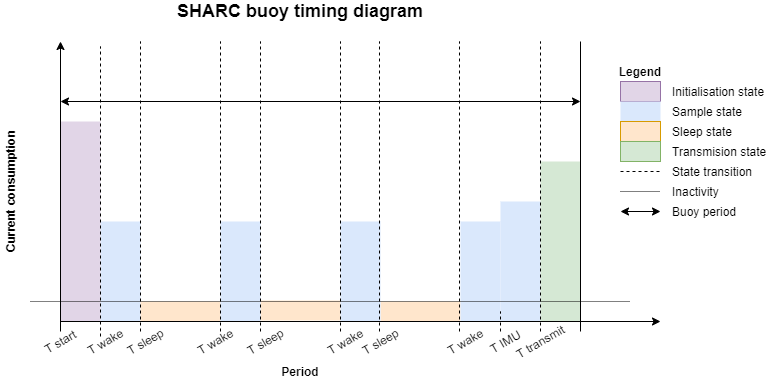
\includegraphics[width=\textwidth]{buoy activity diag.png}
	\caption{Timing diagram for the SHARC buoy showing the sequence and states as well as the expected current draw. The cycle begins with (purple) an initialisation phase where the sensors are verified and configured into the correct modes. Then (blue) the sample periods where the sensors are sampled followed by (orange) a period of inactivity. After four sample sessions, (green) the transmission state is entered where data are condensed into packets and transmitted. Diagram is a representation of the estimated current VS timing and is not to scale. }
	\label{fig:buoyactivity diagram}
\end{figure}

Figure \ref{fig:buoyactivity diagram} shows that the largest current consumption is expected to occur at start up. This is due to the large start up current of the Iridium modem (see Table \ref{tab:ir_specs}). The device is also expected to consume more current during the transmission period. Once again, this is attributed to the power characteristics of the Iridium modem. Finally, the buoy is expected to be inactive for periods relatively longer than the periods of activity. This is dependent on the signal acquisition time of the GPS receiver (see Table \ref{tab:neo7}) as well as the time taken to complete a transmission. The firmware is therefore developed to ensure careful tracking of state transitions and timings to ensure activities are completed in ordered sequence. Finally the fourth state will be the longest period of activity since this is when the IMU will be sampled.
\section{Data flow}
\label{sec:data_flow}

Based on the information above, drift data are collected every half an hour with a transmission occurring after four sampling intervals. The software interfaces with the GPS, environment sensor and power monitor sensor to create a single drift measurement. Since its important to understand the environmental conditions and give an update on the power performance of the device where possible.Therefore, the order of sampling is layed out as follows

\begin{enumerate}
	\item Activate sensor
	\item Collect data
	\item Order and compress data
	\item Store in memory
\end{enumerate}

This sequence is shown in Figure \ref{fig:sampleflow} below.

\begin{figure}[H]
	\centering
	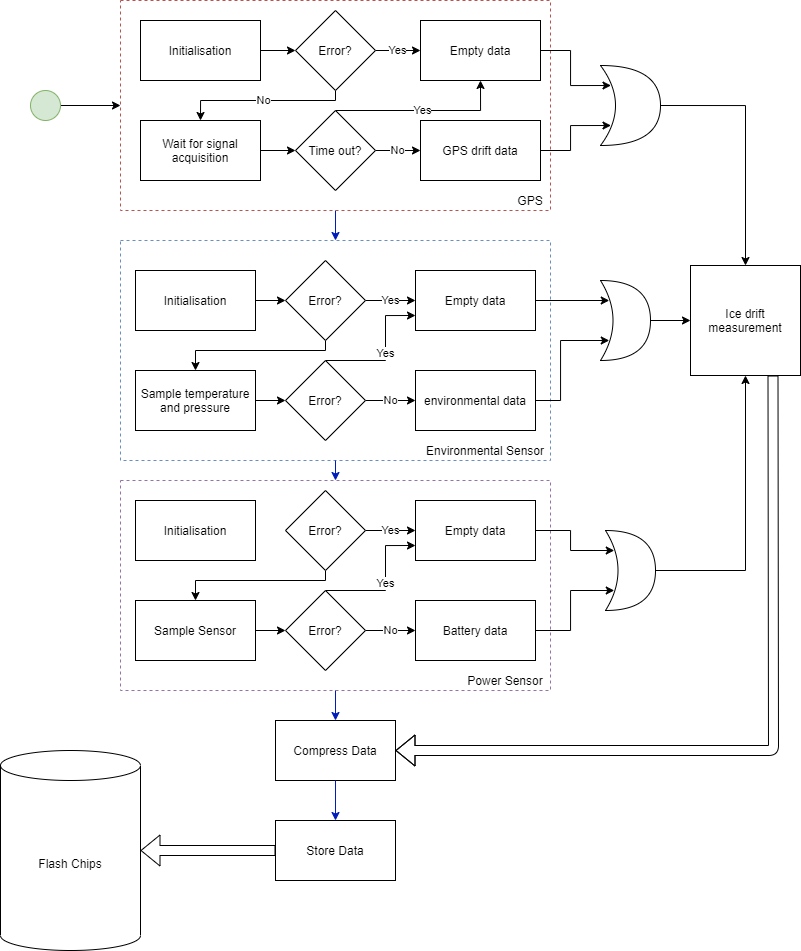
\includegraphics[width = \textwidth]{Sample state flow.png}
	\caption{Flow chart showing the ice drift sampling routine called during the sample state. This diagram contains arrows showing: (blue) the main flow and sequence of steps in the routine, (black) the flow of steps for sampling data from sensors. (white) the flow of data from temporary storage (as an ice drift measurement) to permanent storage. Also shown are (red) GPS subsystem, (blue) environmental sensor and (purple) power sensor.}
	\label{fig:sampleflow}
\end{figure}

The total data collected during a two hour sample period is 140 bytes. The Iridium modem has a maximum transmission buffer of 340 bytes. Therefore, all data can be transmitted at once without any advanced transmission routines required. To accommodate centralised data storage in volatile memory, A custom struct was defined to hold all data in a central location.

\begin{figure}[H]
	\centering
	\begin{lstlisting}
		/*
		* @brief: Structure to store data from GPS in an organised format. Note: custom data types from HAL_GPS.h
		*/
		typedef struct
		{
			uint32_t Etime;			//UTC Epoch representation of time
			Coord_t coordinates;	//GPS coordinates
			Diagnostic_t diag;		//Diagnostic information
			uint32_t env_Temp;		//Environmental temperature
			int32_t atm_Press;		//Atmospheric pressure
			int16_t shunt_v;    //Shunt voltage (mv)
			int16_t bus_v;			//Bus voltage  (mV)
			int16_t current;    //Load current (mA)
			int16_t power;			//Power consumption (mW)
		}GPS_Data_t;
	\end{lstlisting}
	\caption{Data struct for storing drift data collected from the sensors during a sample period where Coord\_t and Diagostic\_t are shown in Appendix \ref{fig:data_coord_t} - \ref{fig:data_Diagnostic_t}} 
	\label{fig:data_drift_struct}
\end{figure}

The struct is populated with data as each sensor completes its sampling. If a sensor fails or is unable to return valid data, the field is left blank and the program continues to sample from other sensors. This ensures that the program is robust when handling sensor fail error to meet the criteria for acceptance test AT004 in Table \ref{tab:AT004}. Once the sensors have finished sampling, the data are condensed into a packet structure and stored in memory. The diagram below shows the structure of a single packet.

\begin{figure}[H]
	\centering
	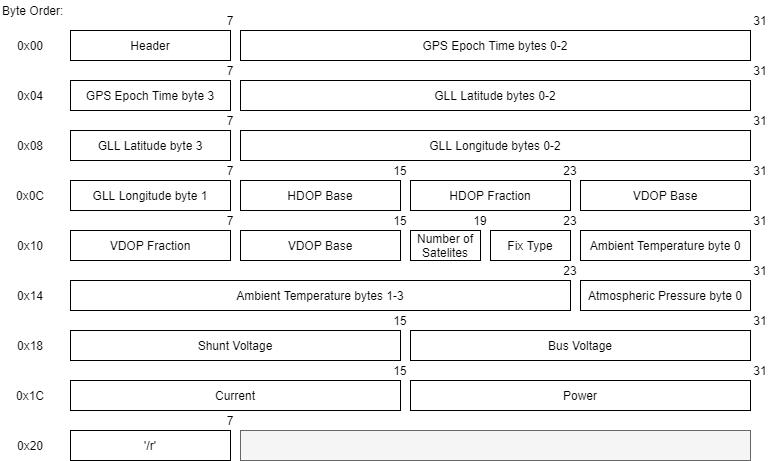
\includegraphics[scale=0.4]{Drift Packet Diagram.png}
	\caption{Diagram showing the structure of a drift data packet including byte position, size and data being collected}
	\label{fig:packet_structure}
\end{figure}

Each packet begins with a header. This is an 8-bit value to give information about the data in the payload. This value consist of a 4-bit identifier (0x0 for drift data) as well as a 4-bit number indicating the sample number (1 to 4) before transmission. Data are stored sequentially in little endian format as shown in Figure \ref{fig:packet_structure} above. A '$\backslash$r' character is used to indicate the end of the packet. This increases the total data requirement from 35 to 37 bytes per sample however, by adding the tail and the header, data integrity is maintained and allow for the standardisation of data transmission.\par 

IMU data, however, is of uniform type therefore, no special structures needed to be created. Data from the IMU is stored in an 8-bit buffer array with the most significant byte of the measurement first. Much like the drift buffer, The data were combined into a packet with a header created at the beginning. The header was given the value 0x57 or \textit{"W"} to identify the packet as an IMU data packet. Then the data occupies the remaining bytes with the final byte of the packet assigned to the '$\backslash$r' character to indicate the end of the packet. \par 

Data are stored in the Flash chips in packet structure form in the first page of the first available Flash chip. Packets are stored sequentially until the device enters transmit state. All data are downloaded from memory and uploaded to the Iridium transmission buffer. The device initiates two transmission sessions. First the drift data are uploaded and transmitted, Then the IMU data. Upon successful transmission, the data are sent via satellite network to the Rock Seven RockBLOCK server. The data are saved to a user's account and sent to their email address where the data can be downloaded as an attachment. The diagram below shows the flow of data from the sensors to the user.

\begin{figure}[H]
	\centering
	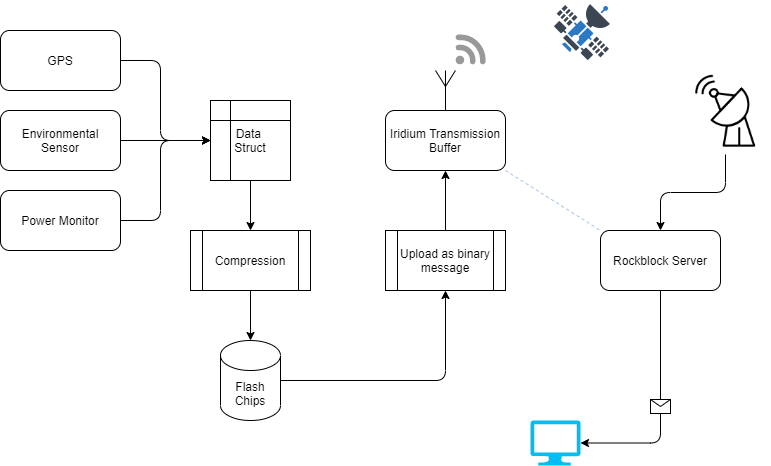
\includegraphics[scale = 0.5]{Data Flow Diagram.png}
	\caption{Diagram showing the flow of data during a cycle of the buoy. The data are sampled by the sensors and converted into packet form where it is stored until it is ready to be transmitted. The transmitted data arrives at a server and is sent via email to the user.}
	\label{fig:data_flow}
\end{figure}

\section{Conclusion}

In conclusion, a robust set of firmware was designed to sequence and control the sensors in a time critical manner. Furthermore, the communication methods of each module were outlined with strategies shown to facilitate communication and manage the flow of data. Firmware validation and full system testing will be discussed in the next Chapter.